% ECIR 2027 FULL paper submission (pivoted from short paper 2026-07-10;
% full-paper scope pending mentor sign-off -- revert to short-paper scope if
% preferred) -- double-anonymous review. Deadline: Oct 5, 2026 (earlier than
% the short-paper deadline of Oct 12) -- more page budget for the mechanism
% story (collapse localization, hourglass connection, VisualNews generality
% check), not more time.
% Author/affiliation block below is intentionally anonymized for review; the real
% author/institution/acknowledgments block is kept in main_camera_ready_authors.tex.inc
% (not created until after acceptance) so this file does not need a rewrite later --
% just swap the \author{...}\institute{...} block and add the Acknowledgments section back.
%
% NOTE: named block below is temporarily in place for supervisor (Yubao) review only --
% swap back to the anonymized block (see ANONYMIZED FOR SUBMISSION comment) before any
% actual double-anonymous ECIR submission.
\documentclass[runningheads]{llncs}
\usepackage[T1]{fontenc}
\usepackage{graphicx}
\usepackage{booktabs}
\usepackage{amsmath}
\usepackage{amssymb}
\usepackage{url}
\setlength{\textfloatsep}{8pt plus 2pt minus 2pt}
\setlength{\intextsep}{6pt plus 2pt minus 2pt}
\setlength{\floatsep}{6pt plus 2pt minus 2pt}
\setlength{\abovecaptionskip}{4pt}
\setlength{\belowcaptionskip}{2pt}

\begin{document}

\title{No Free Lunch for Codebook Balance: Regularization Trade-offs in Generative Multimodal Retrieval}

\titlerunning{No Free Lunch for Codebook Balance}

\author{Tea Cetojevic Tisaj}
\authorrunning{T. Cetojevic Tisaj}
\institute{IRLab Internship, University of Amsterdam \\
Supervised by Prof.\ Maarten de Rijke \& Yubao Tang \\
April--July 2026}

\maketitle

\begin{abstract}
GENIUS and other generative multimodal retrievers decode a discrete semantic ID -- from a residual quantizer (RQ) -- instead of dense nearest-neighbor search, making retrieval cost independent of corpus size. We reproduce GENIUS end-to-end from its officially released Stage-1 checkpoint, then study whether regularizing the RQ codebook toward balanced usage helps or hurts retrieval, via a controlled, multi-seed experiment across MSCOCO, VisualNews (broad-domain), and FashionIQ (fine-grained). On MSCOCO, strong regularization significantly improves mean text-to-image Recall@1 ($23.33\%$ vs.\ $20.78\%$, five decoder seeds, $+12.3\%$ relative, Welch's $t$-test $p<10^{-6}$), but reliably collapses image-to-text Recall from $10.30\%$ to near zero on the identical checkpoints. Since both effects could be artifacts of the single RQ tokenizer each condition was built from, we independently retrained the tokenizer twice more: across three fully independent tokenizers, every regularized one still beats every vanilla one on text-to-image ($24.32\%$ vs.\ $21.16\%$ mean, non-overlapping), and the collapse holds on all three. A dense, decoder-free probe over the frozen tokenizer's embeddings shows the same collapse before any decoder training, partially explained by text embeddings' greater anisotropy under regularization. On VisualNews, the same probe shows both effects are tokenizer-level too, but text-to-image reverses: strong regularization more than halves Recall instead of raising it, while image-to-text collapses exactly as on MSCOCO -- the collapse is architectural and generalizes, the gain is real but dataset-specific. FashionIQ is hurt by any regularization. The natural fix -- decoupling regularization per target modality, including regularizing only the text side -- fails regardless of which side carries the weight: image-to-text stays collapsed even at zero text-side weight, and text-to-image gets worse than either baseline, because image and text rows share one encoder and codebook. No single balance-regularization strategy transfers across retrieval regimes, and even the one clear positive result does not generalize beyond the dataset where we found it.

\keywords{Generative retrieval \and Residual quantization \and Semantic IDs \and Multimodal retrieval \and Codebook balance}
\end{abstract}

\section{Introduction}
\label{sec:intro}

Generative retrieval replaces nearest-neighbor search over dense embeddings with autoregressive generation of a discrete identifier that points directly to the target candidate~\cite{tay2022dsi} (see~\cite{li2024survey} for a survey). GENIUS~\cite{kim2025genius} applies this to universal multimodal search: a residual quantizer (RQ)~\cite{lee2022rqvae} assigns every candidate a short sequence of discrete codes, and a decoder learns to generate a query's target code sequence directly, retrieving in time independent of corpus size. Since the code sequence is the only channel through which a candidate's identity survives into the decoder, codebook quality is a ceiling on what the rest of the system can achieve.

A natural lever for improving it is \emph{balance regularization}: an auxiliary loss discouraging a small subset of codes from absorbing most assignments. Whether this helps is not obvious a priori: broader usage should reduce collisions, but it pulls the encoder from the pure-reconstruction optimum, and its effect may depend on task structure -- a diverse pool may benefit from spreading code usage, while a pool of near-duplicates may instead need the encoder to preserve the subtle differences any diversity pressure would blur.

We first reproduce GENIUS end-to-end from its officially released Stage-1 checkpoint (Section~\ref{sec:setup}), before studying any regularization variant. We then test balance regularization across three regimes -- MSCOCO and VisualNews (broad-domain captioning, two different image/text distributions) and FashionIQ (fine-grained composed fashion retrieval) -- training RQ tokenizers under multiple balance strengths per dataset, with a multi-seed check on every headline number that has already caught one single-run artifact in this exact study (Section~\ref{sec:limitations}), including the decoupling experiment of Section~\ref{sec:direction-aware}, whose constrained-decoding evaluation initially failed on every retrain attempt for reasons we root-cause, fix, and then verify at 3 seeds (Section~\ref{sec:limitations}). Concretely, we ask:

\begin{itemize}
\item \textbf{RQ1:} Which ID-structure properties (codebook utilization, collision rate, reconstruction quality) track downstream retrieval, and is that relationship consistent across retrieval regimes? (Section~\ref{sec:rq1})
\item \textbf{RQ2:} Does balance regularization improve downstream Recall, and at what strength? (Section~\ref{sec:rq2rq3})
\item \textbf{RQ3:} Is the answer stable -- across retrieval direction, across datasets, and under a per-modality decoupling of the regularizer? (Sections~\ref{sec:rq2rq3}--\ref{sec:generality})
\end{itemize}

\paragraph{Contribution.} On MSCOCO, the regularization that \emph{significantly improves} text-to-image retrieval simultaneously destroys image-to-text retrieval on the same dataset. This holds on two independent axes of verification: 5 decoder seeds on the original tokenizer (non-overlapping distributions, $p<10^{-6}$ -- a conclusion that itself survived a scare, Section~\ref{sec:limitations}), and 3 fully independent RQ tokenizers retrained from scratch (every regularized tokenizer outperforms every unregularized one on text-to-image, and the image-to-text collapse holds on all three). We localize this collapse directly to the tokenizer using a dense, decoder-free probe, and partially explain it via text embeddings' greater anisotropy under regularization. Testing generality on VisualNews shows the collapse reproduces cleanly on a second broad-domain corpus, while the text-to-image effect \emph{reverses} -- strong regularization there substantially \emph{hurts} T$\to$I instead of helping it (a $53\%$ relative drop, seed-stable but not significance-tested, unlike MSCOCO's result) -- showing the collapse is an architectural property while the T$\to$I effect is dataset-specific in a way the broad/fine-grained axis alone does not capture. FashionIQ shows any regularization hurts fine-grained retrieval outright. So this study's one confirmed retrieval benefit is real but narrow: significant and tokenizer-verified on MSCOCO, reliably absent or reversed everywhere else we tested.

We then test the natural fix to the trade-off -- decoupling regularization strength per target modality -- at three settings, including regularizing only the image side and, symmetrically, only the text side. It fails on all three: image-to-text retrieval stays collapsed even at zero text-side loss weight, collapses just as completely when text-side weight alone is nonzero, and text-to-image retrieval becomes \emph{worse} than either baseline in every asymmetric setting. This is architectural, not a tuning failure -- image and text rows share one encoder and one EMA-updated codebook, so a modality's loss weight cannot shield its code structure from the other's regularization -- supported by direct evidence of cross-modal code restructuring under zero cross-modal loss weight, and corroborated at the tokenizer level by the same decoder-free probe used to localize the main collapse.

This paper reproduces GENIUS end-to-end, then generalizes and analyzes one of its core design choices across regimes it was never evaluated under. To our knowledge, no prior work has localized an image-to-text collapse in a generative multimodal retriever to the tokenizer rather than the decoder with a direct probe, replicated across two broad-domain corpora, where the same probe also shows VisualNews's text-to-image \emph{drop} is tokenizer-level too -- neither direction is decoder-introduced. Nor has prior work shown the effective regularization strategy for RQ-based semantic IDs is retrieval-regime-dependent in a way that is not simply ``broad vs.\ fine-grained'' -- a single dataset's positive result does not license a general recommendation. And, at 3-seed and tokenizer-level verification (Section~\ref{sec:limitations}), no prior work has shown that per-modality decoupling of a generative retriever's codebook regularization is undermined by the architecture itself, not by tuning.

\section{Background and Related Work}
\label{sec:background}

\paragraph{Generative retrieval.} Generative retrieval replaces nearest-neighbor search with directly decoding an identifier for the target document. DSI~\cite{tay2022dsi} memorizes query-to-docid mappings in a Transformer's parameters; NCI~\cite{wang2022nci} and SEAL~\cite{bevilacqua2022seal} improve the identifier scheme via hierarchical clustering and document substrings; GENRE~\cite{decao2021genre} introduces constrained decoding over a trie of valid identifiers, adopted by nearly every later generative retriever including GENIUS. A parallel line replaces these with \emph{learned discrete semantic IDs}: TIGER~\cite{rajput2023tiger} applies RQ-VAE-style IDs to recommendation, GenRet~\cite{sun2023genret} learns the identifier scheme jointly with retrieval, and IRGen~\cite{zhang2023irgen} applies a similar idea to image retrieval; effectiveness degrades sharply with corpus size and task diversity~\cite{pradeep2023scale} (Section~\ref{sec:setup}; survey:~\cite{li2024survey}). GENIUS~\cite{kim2025genius} is the multimodal instance of this line. None of this prior work studies whether a semantic-ID codebook's balance regularization helps or hurts \emph{retrieval} -- the gap this paper closes.

\paragraph{RQ and the GENIUS pipeline.} An RQ turns a continuous embedding into discrete codes by quantizing in stages~\cite{lee2022rqvae}: each level's codebook finds the nearest of $K$ reference vectors to the residual left by the levels above it. GENIUS~\cite{kim2025genius} applies this to multimodal retrieval over M-BEIR~\cite{wei2024uniir}: a CLIP-style~\cite{radford2021clip} encoder (CLIP-SF) produces a joint image/text embedding; an 8-level RQ (plus a modality-indicator level) quantizes it into a semantic ID; a T5~\cite{raffel2020t5} decoder generates a target ID via constrained beam search over a trie of valid candidate IDs, following~\cite{decao2021genre} -- a prefix tree containing exactly the sequences that name a real candidate, so decoding can never emit a nonexistent ID. Each codebook is fit via an EMA update -- a running average of the embeddings assigned to it, rather than a gradient-trained parameter -- to whatever vectors it observes, with no term rewarding even code usage.

\paragraph{Codebook balance and collapse.} Vector-quantized models suffer \emph{codebook collapse}: a small code subset absorbs most assignments while the rest receive vanishing gradient~\cite{vandenoord2017vqvae}; the standard remedy adds an entropy-style auxiliary loss alongside reconstruction~\cite{zhang2023regularizedvq} -- \emph{balance regularization}. An alternative line avoids collapse by construction rather than regularizing it away: FSQ~\cite{mentzer2024fsq} quantizes each embedding dimension independently, and SimVQ~\cite{zhu2024simvq} reparameterizes the codebook through a single linear layer over a shared basis; we study balance regularization specifically because it is what GENIUS's released architecture uses, not because it is the only remedy to collapse. Concurrent recommendation work reports a related ``hourglass'' code concentration~\cite{kuai2024hourglass} and decouples reconstruction from distribution-matching \emph{within one item stream}~\cite{wang2026decoupledrq}; we instead decouple \emph{across} a cross-modal retriever's two target modalities, failing for a different, architecture-specific reason (Section~\ref{sec:direction-aware}). LETTER~\cite{wang2024letter} adds a diversity loss to RQ-VAE codebooks for generative recommendation -- the closest prior use of our exact intervention -- as one term in a joint objective for a single-modality identifier, not studying its effect on a codebook serving two target modalities. None of this prior work reports whether balance regularization helps or hurts \emph{retrieval}, or whether its effect is stable across regimes -- the gap this paper closes.

\section{Experimental Setup}
\label{sec:setup}

\paragraph{Datasets as contrasting regimes.} We train and evaluate on MSCOCO~\cite{lin2014mscoco}, FashionIQ~\cite{wu2021fashioniq}, and VisualNews~\cite{liu2021visualnews} independently. MSCOCO and VisualNews are both broad-domain captioning retrieval (text-to-image, image-to-text) with diverse pools, but drawn from different image/text distributions (everyday object photography vs.\ news photography and captions); FashionIQ is composed retrieval (image + modification text $\to$ target image) in one narrow domain, its pool dense with visually similar garments. We never compare absolute Recall across datasets, only relative effects within each.

\paragraph{Pipeline, controls, and metrics.} For each dataset we fix the CLIP-SF encoder, extract candidate embeddings once, then train RQ tokenizers differing only in balance strength $\lambda$ -- four points $\{0, 0.3, 1.0, 3.0\}$ (vanilla/weak/medium/strong) for MSCOCO and FashionIQ, and the two most informative points $\{0, 3.0\}$ for VisualNews (Section~\ref{sec:generality}) -- holding fixed the RQ architecture, level count, codebook size (4096), the T5 retriever, and all splits/decoding settings (50-beam constrained search). The grid is approximately log-spaced from no regularization to a strength at which the balance term dominates ID structure (Table~\ref{tab:table1}); we did not sweep further points given the per-point training cost of a from-scratch RQ tokenizer and retriever. Each tokenizer's IDs retrain the same retriever from scratch. We measure \emph{ID-structure} (utilization, collision rate, reconstruction MSE/cosine similarity) and \emph{retrieval} Recall@1/5/10 on held-out test splits via the real GENIUS pipeline -- T5 + constrained beam search over the correct test pool, not a dense-embedding proxy. As context for every absolute number that follows: a dense CLIP-SF baseline with no RQ and no decoder reaches T$\to$I $55.50\%$/I$\to$T $74.00\%$ Recall@1 on the same MSCOCO pools -- discretizing into a semantic ID pays a large toll in exchange for $O(1)$-cost retrieval~\cite{tay2022dsi,pradeep2023scale}, and every regularization effect we study operates well below this ceiling.

\paragraph{Seed verification.} Every headline Recall number is a mean over multiple training seeds for the retriever (Stage 2), holding the RQ tokenizer (Stage 1) fixed per variant: 3 seeds by default, extended to 5 for MSCOCO vanilla/strong specifically after a seed-count stress test (Section~\ref{sec:rq2rq3}). ID-structure/correlation statistics (Section~\ref{sec:rq1}) come from the single tokenizer per variant ($n=4$ per dataset) and are descriptive only. To separate genuine seed variance from eval-time noise, we independently re-ran evaluation on fixed MSCOCO checkpoints: vanilla/strong (well-conditioned codebooks) matched to four decimal places across two independent repeats, indicating negligible eval-repeat variance under normal conditions. img3txt0p3 (a severely collapsed codebook, Section~\ref{sec:direction-aware}) instead showed small but real run-to-run drift across three independent evals (T$\to$I R@1 $5.40\%/5.45\%/5.41\%$) -- consistent with, not contradicting, the fp16 beam-search near-tie mechanism Section~\ref{sec:limitations} uses to explain that variant's decode-crash nondeterminism.

\paragraph{Reproducing GENIUS, before studying it.} Before running any balance-regularization variant, we first reproduce the released system itself: GENIUS's officially released \emph{Stage-1 RQ checkpoint} paired with our own Stage-2 decoder, trained on the full $\sim$1.3M-query M-BEIR union across 16 tasks (the officially released decoder weights are not public). Table~\ref{tab:reproduction} compares our reproduction against the paper's published numbers.

\begin{table}[t]
\centering
\caption{Reproducing GENIUS's released Stage-1 checkpoint with our own union-trained Stage-2 decoder, vs.\ the original paper's published numbers.}
\label{tab:reproduction}
\footnotesize
\begin{tabular}{@{}llrr@{}}
\toprule
Dataset & Metric & Published & Reproduced \\
\midrule
FashionIQ & R@10 (no rerank) & $13.1\%$ & $18.3$--$18.6\%$ \\
FashionIQ & R@10 (reranked)  & $19.2\%$ & -- \\
MSCOCO    & T$\to$I R@1      & $40.1\%$ & $8.1\%$ \\
\bottomrule
\end{tabular}
\end{table}

FashionIQ reproduces in the right range without reranking, evidence the pipeline itself is correct. MSCOCO does not: $8.1\%$ against the published $40.1\%$, consistent with capacity dilution across 16 tasks~\cite{pradeep2023scale} plus our lack of validation-based checkpoint selection and hard negatives -- training-recipe gaps we disclose rather than paper over, not architecture or codebase failures. \emph{This paper's own numbers} are lower still, for a different, deliberate reason: every variant here trains a \emph{fresh} RQ tokenizer and decoder independently per dataset (above), isolating $\lambda$ as the only difference rather than exposure to the union's larger, more diverse training distribution. The comparison this paper relies on throughout -- vanilla vs.\ weak/medium/strong \emph{within} that same from-scratch, single-dataset regime -- is unaffected by either gap, since every variant in it is trained identically apart from $\lambda$.

\section{RQ1: Which ID-Structure Properties Track Retrieval?}
\label{sec:rq1}

\begin{table}[t]
\centering
\caption{ID-structure properties by balance strength $\lambda$, both datasets.}
\label{tab:table1}
\footnotesize
\begin{tabular}{@{}llrrrr@{}}
\toprule
Dataset & $\lambda$ & Utilization & Collision & Recon.\ MSE & Cosine sim.\\
\midrule
MSCOCO    & 0.0 (vanilla) & 57.7\% & 0.87\% & 0.000124 & 95.2\% \\
MSCOCO    & 0.3 (weak)    & 55.9\% & 6.38\% & 0.000647 & 75.1\% \\
MSCOCO    & 1.0 (medium)  & 63.4\% & 22.7\% & 0.000974 & 62.6\% \\
MSCOCO    & 3.0 (strong)  & 68.2\% & 69.7\% & 0.000954 & 63.4\% \\
\midrule
FashionIQ & 0.0 (vanilla) & 18.4\% & 4.18\% & 0.000037 & 98.6\% \\
FashionIQ & 0.3 (weak)    & 10.7\% & 4.37\% & 0.000255 & 90.2\% \\
FashionIQ & 1.0 (medium)  & 11.6\% & 4.45\% & 0.000310 & 88.1\% \\
FashionIQ & 3.0 (strong)  & 11.6\% & 4.45\% & 0.000386 & 85.2\% \\
\midrule
VisualNews & 0.0 (vanilla) & 53.2\% & 0.43\% & 0.000098 & 96.2\% \\
VisualNews & 3.0 (strong)  & 55.0\% & 1.00\% & 0.000610 & 76.6\% \\
\bottomrule
\end{tabular}
\end{table}

Stronger $\lambda$ \emph{increases} MSCOCO utilization (57.7\%$\to$68.2\%) while \emph{degrading} reconstruction (cosine similarity 95.2\%$\to$63.4\%); FashionIQ shows the opposite sign on utilization (18.4\%$\to$11.6\%) while still degrading reconstruction. Correlating each metric against headline Recall@1 ($n=4$ per dataset, Pearson $r$, descriptive only) sharpens this: on MSCOCO, collision rate correlates \emph{positively} with Recall ($r{=}{+}0.79$) -- the worst-reconstruction, highest-collision configuration (strong) achieves the best Recall. On FashionIQ, utilization is the strongest predictor, also positive ($r{=}{+}0.90$), while collision and MSE correlate negatively ($r{=}{-}0.70$, $r{=}{-}0.75$) -- the conventional ``better reconstruction $\to$ better retrieval'' story holds here but not on MSCOCO. No ID-structure metric predicts Recall with a consistent sign across both regimes; the collapse-mitigation metrics from Section~\ref{sec:background} are, at best, incomplete and dataset-dependent proxies for retrieval quality. Strong's 69.7\% collision rate raises a natural concern: our retrieval pipeline breaks ties within an identical ID by candidate-pool file order (not similarity), so part of its Recall could be ordering luck rather than genuine discrimination. We checked directly: reconstructing each query's full tie group from its top-predicted code, expected R@1 under a random within-group tie-break (23.31\%) and even the adversarial worst case (23.29\%) both sit within 0.05 points of strong's reported 23.33\% (vanilla: 20.84\%/20.83\% vs.\ 20.86\%) -- whenever a query's gold candidate is reachable via its top-predicted code at all, that code is essentially always a singleton for that query. The collision-heavy codes are populated by candidates that rarely serve as anyone's gold target, so file-order tie-breaking is not inflating the headline gain.

\paragraph{VisualNews barely restructures under the same $\lambda$, yet its Recall swings hardest.} VisualNews was tested only at $\{0,3.0\}$ (Section~\ref{sec:generality}), too few points for a correlation, but the contrast with MSCOCO is stark on its own: strong regularization moves VisualNews's utilization by only $+1.8$ points ($53.2\%\to55.0\%$) and collision by $+0.6$ points ($0.43\%\to1.00\%$) -- an order of magnitude smaller shift than MSCOCO's ($+10.5$ and $+68.8$ points respectively) -- while reconstruction still degrades comparably (cosine similarity $96.2\%\to76.6\%$). Yet VisualNews's T$\to$I Recall swings by $53\%$ relative (Section~\ref{sec:generality}), \emph{larger} than MSCOCO's $+12.3\%$ gain. ID-structure disruption and retrieval-effect magnitude are not just inconsistently signed across datasets (above) -- they are not even consistently \emph{sized}: the dataset with the smallest codebook restructuring shows the largest Recall effect.

\paragraph{The hourglass phenomenon is induced by regularization, and only on MSCOCO.} Kuai et al.~\cite{kuai2024hourglass} report intermediate RQ levels concentrating relative to boundary levels (``hourglass'') in recommendation-system semantic IDs. We measure this directly: for each variant, the mean relative entropy of levels 2--7 minus that of levels $\{1,8\}$ (negative = hourglass shape). On MSCOCO this score moves from $+0.03$ (vanilla, no hourglass) to $-0.37$ (strong, pronounced hourglass) monotonically with $\lambda$ -- balance regularization \emph{induces} the hourglass shape here, rather than merely failing to prevent it. On FashionIQ the score stays within $[-0.02, +0.20]$ across all four variants, never developing an hourglass shape regardless of $\lambda$. This is a third, independent facet of the same dataset-dependence this paper documents throughout, and the first empirical connection between balance regularization and the hourglass phenomenon reported in a different (single-stream, recommendation) setting.

\section{RQ2/RQ3: The Balance Trade-off, and Its Reversal Across Regimes}
\label{sec:rq2rq3}

\begin{table}[t]
\centering
\caption{Retrieval Recall by balance strength, mean $\pm$ std across seeds (headline: T$\to$I for MSCOCO, IT$\to$I for FashionIQ; other dir.: I$\to$T, MSCOCO only). MSCOCO vanilla/strong $n{=}5$ (seed 2023 re-evaluated, Section~\ref{sec:limitations}); weak/medium R@1 $n{=}3$.}
\label{tab:table2}
\scriptsize
\setlength{\tabcolsep}{3.2pt}
\begin{tabular}{@{}llrrrr@{}}
\toprule
Dataset & $\lambda$ & Headline R@1 & Headline R@5 & Headline R@10 & Other dir.\ R@1 \\
\midrule
MSCOCO & 0.0 (vanilla) & 20.78 $\pm$ 0.06 & 41.62 $\pm$ 0.09 & 52.37 $\pm$ 0.19 & \textbf{10.30 $\pm$ 0.67} \\
MSCOCO & 0.3 (weak)    & 14.13 $\pm$ 0.53 & 30.89 $\pm$ 0.05 & 40.37 $\pm$ 0.10 & 0.05 $\pm$ 0.02 \\
MSCOCO & 1.0 (medium)  & 10.36 $\pm$ 0.69 & 24.11 $\pm$ 0.12 & 32.44 $\pm$ 0.05 & 0.03 $\pm$ 0.01 \\
MSCOCO & 3.0 (strong)  & \textbf{23.33 $\pm$ 0.11} & 47.41 $\pm$ 0.18 & 58.74 $\pm$ 0.11 & 0.03 $\pm$ 0.02 \\
\midrule
FashionIQ & 0.0 (vanilla) & \textbf{0.61 $\pm$ 0.10} & $2.94\pm0.02$ & $4.76\pm0.05$ & -- \\
FashionIQ & 0.3 (weak)    & 0.27 $\pm$ 0.06 & $1.16\pm0.14$ & $1.82\pm0.15$ & -- \\
FashionIQ & 1.0 (medium)  & 0.21 $\pm$ 0.09 & $0.94\pm0.13$ & $1.60\pm0.10$ & -- \\
FashionIQ & 3.0 (strong)  & 0.25 $\pm$ 0.08 & $1.03\pm0.09$ & $1.60\pm0.10$ & -- \\
\bottomrule
\end{tabular}
\end{table}

\paragraph{The MSCOCO T$\to$I gain is real: we chased a decode-time artifact, not the effect.} We stress-tested this paper's headline number three times. The single-seed estimate ($+50.9\%$) narrowed to $+22.0\%$ at 3 seeds; 2 more seeds (5 total) at first appeared to erase it ($p{=}0.057$) because vanilla's seed-2023 point was a $\sim$6-point outlier from its own other 4 seeds. Re-evaluating that one point (identical checkpoint and config, prompted by a separate R@5/R@10 anomaly, Section~\ref{sec:limitations}) corrected it $14.08\%\to20.86\%$ -- squarely inside vanilla's other-seed cluster ($20.70$--$20.81\%$) -- and the corrected comparison is decisive: strong $23.33\pm0.11\%$ vs.\ vanilla $20.78\pm0.06\%$, non-overlapping $\pm1$-std bands, $p<10^{-6}$ (Welch's $t$-test). The gain is $+12.3\%$ ($2.55$ points), smaller than the original estimate but resting on the most scrutinized number in this paper rather than the least. On FashionIQ, vanilla wins outright; the ranking among weak/medium/strong is \emph{not} seed-stable (medium's own seed range, $0.13$--$0.42\%$, exceeds the gap between any pair), so we report only ``vanilla wins.''

\paragraph{The gain survives retraining the tokenizer itself, not just the decoder.} Every number above holds the Stage-1 RQ tokenizer fixed; since Table~\ref{tab:localization} shows both effects are tokenizer-level, Stage-1 training variance itself was unmeasured. We trained 2 more fully independent Stage-1 tokenizers per condition (seeds 7, 13), each with one Stage-2 decoder (seed 2023) on top. Across 3 independent tokenizers, T$\to$I R@1 is vanilla $20.86\%/21.70\%/20.91\%$ (mean $21.16\pm0.47$) vs.\ strong $23.33\%/24.87\%/24.75\%$ (mean $24.32\pm0.86$) -- every strong tokenizer beats every vanilla one, a non-overlapping gap larger than the original estimate ($3.16$ vs.\ $2.55$ points). I$\to$T is equally robust: vanilla stays high ($10.52\%/10.24\%/9.58\%$), strong stays collapsed ($0.04\%/0.02\%/0.02\%$). Descriptive $n{=}3$, not a further inferential test (as elsewhere, Section~\ref{sec:rq1}) -- but both headline effects now hold across decoder seeds \emph{and} tokenizers.

\begin{figure}[t]
\centering
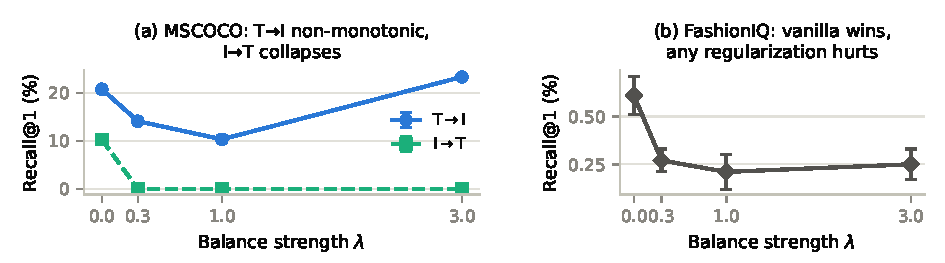
\includegraphics[width=0.98\textwidth]{figures/fig_lambda_recall.pdf}
\caption{Recall@1 vs.\ balance strength $\lambda$, mean $\pm$ std across seeds per point (MSCOCO vanilla/strong: 5 seeds; weak/medium: 3 seeds; FashionIQ: 3 seeds). MSCOCO's T$\to$I curve is non-monotonic -- weak/medium dip below both vanilla and strong -- but vanilla and strong themselves are tight, non-overlapping clusters; I$\to$T collapses immediately past $\lambda=0$; FashionIQ falls immediately and stays low at every regularized $\lambda$.}
\label{fig:lambda-recall}
\end{figure}

\paragraph{The other cost: an image-to-text collapse.} Unlike T$\to$I, I$\to$T is unambiguous and never in doubt across any seed count: vanilla is the \emph{only} variant with working I$\to$T ($10.30\%$ mean, 5 seeds, std $0.67$); all regularized variants collapse to $\leq 0.05\%$ mean, seed-independently, with std an order of magnitude smaller than vanilla's own. We ruled out two candidate mechanisms as sufficient explanations: a stale constrained-decoding trie (corrected; collapse persisted after the fix), and modality-code collapse alone (vanilla and weak collapse to an \emph{identical} degenerate modality-indicator pattern, yet only vanilla's I$\to$T works).

\begin{table}[t]
\centering
\caption{Localizing the collapse: a dense, no-T5 probe (cosine similarity over the frozen RQ's quantized embedding, no beam search, no trie) against the real T5+beam-search pipeline, same checkpoints.}
\label{tab:localization}
\footnotesize
\begin{tabular}{@{}lrrrr@{}}
\toprule
Variant & Dense T$\to$I R@1 & Dense I$\to$T R@1 & Real T$\to$I R@1\textsuperscript{*} & Real I$\to$T R@1\textsuperscript{*} \\
\midrule
vanilla & 26.65\% & \textbf{7.52\%} & 20.78\% & \textbf{10.30\%} \\
weak    & 17.32\% & 0.04\% & 14.13\% & 0.05\% \\
medium  & 12.87\% & 0.00\% & 10.36\% & 0.03\% \\
strong  & 24.23\% & 0.02\% & 23.33\% & 0.03\% \\
\bottomrule
\end{tabular}
\\[2pt]
\footnotesize\textsuperscript{*}multi-seed R@1 mean (Table~\ref{tab:table2}); the dense probe uses the single frozen Stage-1 RQ checkpoint shared by all Stage-2 seeds, so no seed mismatch is introduced by this comparison.
\end{table}

\paragraph{Localizing the collapse: tokenizer, not decoder.} Table~\ref{tab:localization} answers the open question directly: the dense probe involves no T5, no beam search, no trie -- just cosine similarity over the frozen RQ's quantized embedding. I$\to$T \emph{already} collapses here for weak/medium/strong ($\leq 0.04\%$, matching the real pipeline's band), while vanilla's dense I$\to$T ($7.52\%$) stays far above chance, in the same range as its real-pipeline number ($10.30\%$ mean). T$\to$I shows the opposite pattern: all four variants retain substantial, rank-correlated dense recall, consistent with T5 doing comparable real work here. Balance regularization degrades the RQ embedding space's ability to discriminate text candidates for image queries \emph{before Stage-2 training ever begins}.

\paragraph{A partial answer to \emph{why} text is hit harder: text embeddings start more anisotropic.} On vanilla's fused (pre-quantization) embeddings, text candidates occupy a narrower cone than image candidates (mean pairwise cosine similarity, the standard anisotropy measure~\cite{ethayarajh2019anisotropy,gao2019degeneration}: $0.842$ vs.\ $0.675$), and under weak/medium regularization text-side level-1 code entropy drops considerably more than image-side (vanilla$\to$medium: text $0.725\to0.457$, a $37\%$ drop, vs.\ image $0.868\to0.778$, a $10\%$ drop) -- consistent with per-sample equidistance pressure shattering an already-narrower text cluster more severely. Not the whole story: at strong $\lambda$, both anisotropy and level-1 entropy partially \emph{recover} toward vanilla's values (text entropy $0.745$, near vanilla's $0.725$) even though I$\to$T stays just as collapsed ($0.02\%$). So anisotropy explains the moderate-$\lambda$ damage, not why the collapse persists at strong $\lambda$ once entropy recovers -- the full mechanism remains open (Section~\ref{sec:limitations}).

\paragraph{Utilization moves in opposite directions.} Reinforcing RQ1, regularization \emph{increases} MSCOCO utilization but \emph{decreases} FashionIQ's, under the identical regularizer, codebook size, and level count -- MSCOCO's diverse pool may have room to spread code usage productively, while FashionIQ's dense, near-duplicate pool may already need most capacity for faithful reconstruction. A pool-size confound (FashionIQ's pool is $\approx 9.6\times$ smaller) is controlled for by re-running MSCOCO's diagnostics on a size-matched 74K subsample: MSCOCO subsampled to FashionIQ's size still runs $2$--$4\times$ FashionIQ's utilization with far steeper collision growth, so the domain-dependence finding survives the control.

\section{Direction-Aware $\lambda$: A Natural Fix That Fails Architecturally}
\label{sec:direction-aware}

Section~\ref{sec:rq2rq3}'s trade-off suggests an obvious refinement: regularize only the codes that need it, decoupling the regularizer's strength per target modality ($\lambda_{\text{img}}$/$\lambda_{\text{txt}}$) instead of one shared $\lambda$ (a per-row loss weight, unit-tested to reduce to the existing single-$\lambda$ path when $\lambda_{\text{img}}=\lambda_{\text{txt}}$). We test three settings: \textbf{img3txt0} ($\lambda_{\text{img}}=3.0$, $\lambda_{\text{txt}}=0.0$), \textbf{img3txt0p3} ($\lambda_{\text{img}}=3.0$, $\lambda_{\text{txt}}=0.3$), and \textbf{img0txt3} ($\lambda_{\text{img}}=0.0$, $\lambda_{\text{txt}}=3.0$) -- the mirror-image cell, regularizing \emph{only} the text side, which directly tests whether text-side pressure alone is sufficient to cause the I$\to$T collapse.

\begin{table}[t]
\centering
\caption{Direction-aware $\lambda$ vs.\ the uniform baselines, MSCOCO T$\to$I / I$\to$T Recall@1, mean $\pm$ std across seeds.}
\label{tab:direction-aware}
\footnotesize
\begin{tabular}{@{}lrrrr@{}}
\toprule
Variant & $\lambda_{\text{img}}$ & $\lambda_{\text{txt}}$ & T$\to$I R@1 & I$\to$T R@1 \\
\midrule
vanilla      & 0.0 & 0.0 & 20.78 $\pm$ 0.06\% & \textbf{10.30 $\pm$ 0.67\%} \\
strong       & 3.0 & 3.0 & \textbf{23.33 $\pm$ 0.11\%} & 0.03 $\pm$ 0.02\% \\
img3txt0     & 3.0 & 0.0 & 7.87 $\pm$ 0.12\% & 0.12 $\pm$ 0.04\% \\
img3txt0p3   & 3.0 & 0.3 & 5.56 $\pm$ 0.13\% & 0.13 $\pm$ 0.05\% \\
img0txt3     & 0.0 & 3.0 & 6.53 $\pm$ 0.08\% & 0.03 $\pm$ 0.01\% \\
\bottomrule
\end{tabular}
\\[2pt]
\footnotesize vanilla/strong: 5 seeds (Table~\ref{tab:table2}). img3txt0/img3txt0p3/img0txt3: 3 seeds each -- img3txt0/img3txt0p3 originally failed 12/12 decode attempts (fp16 nondeterminism on concentrated codebooks, Section~\ref{sec:limitations}); a robustness fix resolved it, and all seeds shown completed via valid beam search (img0txt3 hit no such dead-end).
\end{table}

\paragraph{The hypothesis fails on all three counts.} No setting recovers I$\to$T: all three stay collapsed, 3-seed means ($0.12\pm0.04\%$/$0.13\pm0.05\%$/$0.03\pm0.01\%$) -- true even for img3txt0 and img0txt3, each with one loss weight at exactly zero. img0txt3's I$\to$T ($0.03\pm0.01\%$) is numerically indistinguishable from strong's full-regularization collapse ($0.03\pm0.02\%$, no test run given both are thin samples): text-side pressure \emph{alone} collapses I$\to$T as completely as regularizing both sides, the cleanest evidence text-side regularization suffices on its own. T$\to$I is \emph{worse than vanilla} in all three cells ($7.87\%$/$5.56\%$/$6.53\%$ vs.\ $20.78\%$), not merely worse than strong: every asymmetric setting underperforms both baselines, regardless of which side carries the weight.

\begin{figure}[t]
\centering
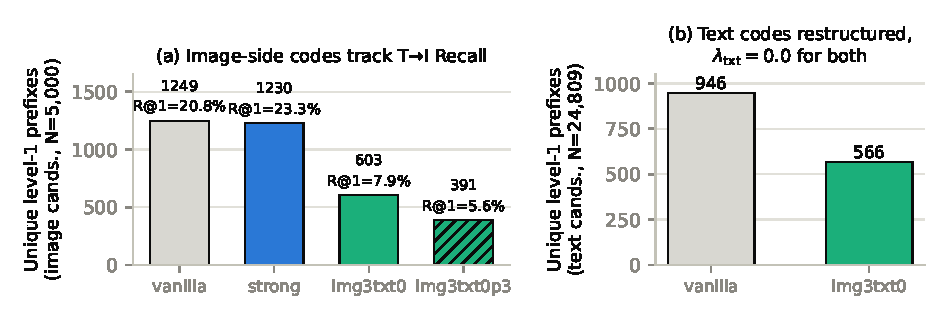
\includegraphics[width=0.92\textwidth]{figures/fig_prefixes.pdf}
\caption{Unique level-1 RQ prefixes by variant -- level-1 is the first token of the semantic ID, the level constrained beam search prunes on first. (a) Image-side count tracks T$\to$I Recall (3-seed mean) almost monotonically. (b) Text-side prefixes, vanilla vs.\ img3txt0 -- both have $\lambda_{\text{txt}}=0.0$, yet img3txt0's text codes are visibly restructured: direct evidence that image-side regularization reaches text-side structure through the shared encoder and codebook.}
\label{fig:prefixes}
\end{figure}

\paragraph{Mechanism: the codebook is not decomposable per modality.} Not an implementation bug: the per-row weight is applied correctly (a shape assertion never fired across training; img3txt0's training loss lands almost exactly half of strong's, as expected if half the rows carry $\lambda=3$ and half carry $\lambda=0$). Zero text-side weight does not protect text-side structure: image and text rows share one encoder forward pass, the same contrastive/reconstruction losses, and one EMA-updated codebook at every level. Figure~\ref{fig:prefixes}(b) shows this directly: under img3txt0, text candidates' codes are measurably restructured relative to vanilla ($566$ vs.\ $946$ unique level-1 prefixes) despite exactly zero text-side loss weight. This also explains the T$\to$I ordering in Figure~\ref{fig:prefixes}(a): unique image-side level-1 codes track T$\to$I Recall almost monotonically -- strong preserves level-1 diversity while flattening mid-levels into constants the decoder learns easily; the asymmetric settings instead concentrate level-1 itself, with no such payoff. Overall, the natural fix is dominated by both uniform-$\lambda$ alternatives on every metric measured -- not because the right combination remains to be tuned, but because a shared encoder and codebook give a per-row loss weight no mechanism to produce a per-modality effect.

\paragraph{Tokenizer-level corroboration.} All three asymmetric variants are Stage-1 checkpoints with no Stage-2 seed involved, so the same decoder-free probe that localized the main I$\to$T collapse (Table~\ref{tab:localization}) runs on them directly. All three collapse on I$\to$T at the tokenizer level ($0.02\%$/$0.02\%$/$0.02\%$ dense R@1, matching weak/medium/strong's $\leq0.04\%$ band, far below vanilla's $7.52\%$), numerically indistinguishable from strong's despite img0txt3's zero image-side weight. The probe also reproduces T$\to$I-worse-than-vanilla for all three ($14.13\%$/$11.81\%$/$8.67\%$ vs.\ vanilla's $26.65\%$); img0txt3's relative ordering differs slightly between dense and decoder-level (worst vs.\ middle), a minor discrepancy noted rather than papered over -- the collapse and worse-than-both-baselines pattern hold regardless. Tokenizer- and decoder-level evidence otherwise agree independently.

\section{Generality: A Third Dataset}
\label{sec:generality}

Sections~\ref{sec:rq2rq3}--\ref{sec:direction-aware} document a striking asymmetry on MSCOCO: balance regularization significantly improves T$\to$I while reliably collapsing I$\to$T on the same checkpoints, and we localize the collapse to the RQ tokenizer itself (Table~\ref{tab:localization}). This raises an obvious question: is the I$\to$T collapse a property of MSCOCO specifically, or of RQ-based semantic IDs whenever text is the target modality, regardless of dataset? We test this on VisualNews, a broad-domain news image-captioning corpus structurally similar to MSCOCO (both T$\to$I and I$\to$T directions, a large and diverse candidate pool) but drawn from an entirely different domain (news photography and captions vs.\ everyday object photography).

\paragraph{Setup.} We extract VisualNews-only local candidate pools and query splits from the M-BEIR union files already used in this project's broader union-training effort, since the original raw VisualNews source dump is not preserved in our environment; this yields 100,000 training image candidates, 99,903 training text candidates, and 99,903/100,000 T$\to$I/I$\to$T training queries. No official M-BEIR held-out test partition exists for VisualNews in our downloaded data; we therefore repurpose the union pool's validation split (19,996/20,000 T$\to$I/I$\to$T queries, never seen during training) as our test set -- a disclosed deviation from the official-test-split convention used for MSCOCO and FashionIQ, not an oversight. We train only the two most informative balance strengths, vanilla ($\lambda=0$) and strong ($\lambda=3.0$), each with the same 3-seed protocol (2023/7/13) used throughout this paper, holding every other pipeline component identical to the MSCOCO/FashionIQ setup.

\begin{table}[t]
\centering
\caption{VisualNews Recall@1 by balance strength, 3-seed mean $\pm$ std.}
\label{tab:visualnews}
\footnotesize
\begin{tabular}{@{}lrr@{}}
\toprule
$\lambda$ & T$\to$I R@1 (mean $\pm$ std) & I$\to$T R@1 (mean $\pm$ std) \\
\midrule
0.0 (vanilla) & \textbf{20.07 $\pm$ 0.11\%} & \textbf{2.88 $\pm$ 0.05\%} \\
3.0 (strong)  & 9.43 $\pm$ 0.08\%  & 0.01 $\pm$ 0.00\% \\
\bottomrule
\end{tabular}
\end{table}

\paragraph{The collapse generalizes; the gain reverses.} VisualNews reproduces one half of the MSCOCO asymmetry cleanly and moves the opposite way on the other, both seed-stable. I$\to$T collapses under strong regularization exactly as on MSCOCO -- from $2.88\%$ to $0.01\%$ ($\text{std}\leq0.05$ points on both variants) -- supporting that this is a general property of shared-codebook RQ tokenizers under per-sample entropy pressure, not an MSCOCO-specific artifact, and strengthening Section~\ref{sec:rq2rq3}'s localization claim. But T$\to$I moves the opposite way from MSCOCO: strong regularization more than \emph{halves} VisualNews's T$\to$I Recall@1 ($20.07\%\to9.43\%$, a $53\%$ relative drop, std $\leq0.11$ points), a large, seed-stable drop (3 seeds, no significance test reported, unlike MSCOCO's Welch's-$t$-backed result) in the direction opposite to MSCOCO's significant $+12.3\%$ gain (Section~\ref{sec:rq2rq3}).

\paragraph{Tokenizer-level corroboration: both directions localize before Stage-2 training.} The same decoder-free probe that localizes MSCOCO's I$\to$T collapse (Table~\ref{tab:localization}) runs directly on VisualNews's vanilla/strong Stage-1 checkpoints. Both effects are already present at the tokenizer level: dense I$\to$T falls $2.67\%\to0.00\%$, matching the real pipeline's $2.88\%\to0.01\%$; dense T$\to$I falls $20.22\%\to10.59\%$ ($\sim$48\% relative), closely tracking the real pipeline's $20.07\%\to9.43\%$ ($\sim$53\%). Neither direction is decoder-introduced -- both are set before Stage-2 training begins, extending Section~\ref{sec:rq2rq3}'s localization to a second corpus and both directions at once.

This means the paper's central trade-off is not simply ``broad-domain wants strong regularization, fine-grained wants none'': MSCOCO and VisualNews are both broad-domain, bidirectional corpora, yet strong $\lambda$ significantly \emph{helps} T$\to$I on one (MSCOCO, Welch's-$t$-verified) and substantially \emph{hurts} it on the other (VisualNews, seed-stable but not significance-tested). The I$\to$T collapse looks like a general architectural property; whatever makes MSCOCO uniquely receptive to a T$\to$I gain looks specific to MSCOCO -- plausibly the particular density or redundancy of its candidate distribution (many near-duplicate captions per image) rather than ``broad domain'' as a category. We flag pinning down what property of MSCOCO's candidate distribution produces this reversal as the most direct follow-up this result motivates.

\section{Discussion, Limitations, and Conclusion}
\label{sec:limitations}

\paragraph{Correlational evidence is descriptive.} Section~\ref{sec:rq1}'s correlations use four $\lambda$ points per dataset; the \emph{sign reversal} between datasets is the finding, not $n=4$ significance.

\paragraph{FashionIQ's small Recall is not noise.} All FashionIQ R@1 values are below $1\%$, but the vanilla-vs-regularized gap holds at R@5/R@10 too, 3-seed mean $\pm$ std (vanilla $2.94\pm0.02\%$/$4.76\pm0.05\%$ vs.\ best regularized, weak, $1.16\pm0.14\%$/$1.82\pm0.15\%$) -- not a $k{=}1$ artifact. The ranking \emph{among} regularized variants is not seed-stable; we claim none.

\paragraph{Seed 2023's original eval was an artifact in R@1, not only R@5/R@10.} Seed 2023's R@5/R@10 originally showed near-flat growth over R@1 (vanilla: $14.08\to18.08\to18.11\%$) vs.\ seeds 7/13/21/42's normal $\sim$2--2.5$\times$ growth -- a truncated ranked list, not a genuine effect. Re-evaluating that point (identical checkpoint and config) also corrected R@1: vanilla moved $14.08\%\to20.86\%$, now consistent with its other four seeds ($20.70$--$20.81\%$) rather than a $\sim$6-point outlier that drove this paper's original $+50.9\%\to+22.0\%\to$``not significant'' narrowing (Section~\ref{sec:rq2rq3}). We ruled out the two likely causes: the checkpoint is unchanged (timestamp-confirmed), and the reused trie passed a hash check against current codes -- not the documented stale-cache bug. The remaining explanation is genuine run-to-run non-determinism in beam-search decoding; disclosed as open, not solved. Corrected values are used throughout (Tables~\ref{tab:table2}--\ref{tab:localization}, Figure~\ref{fig:lambda-recall}).

\paragraph{Remaining open points, and scope.} The I$\to$T collapse is localized to the tokenizer (Section~\ref{sec:rq2rq3}) and partially explained by text embeddings' greater anisotropy under moderate regularization, but not why it persists undiminished at strong $\lambda$ once code entropy partially recovers -- a gap we disclose rather than paper over. The dense-retrieval ceiling of Section~\ref{sec:setup} bounds all variants here, sitting 3--8$\times$ below it and the released model. Our datasets are structurally contrasting exemplars, not a sweep; the optimal $\lambda$ found need not transfer to a further regime. Adapting Wang et al.'s decoupled-RQ design~\cite{wang2026decoupledrq} to our cross-modal setting is out of scope. VisualNews was tested only at $\lambda\in\{0,3\}$; a favorable intermediate strength cannot be excluded.

\paragraph{Direction-aware $\lambda$'s decode crash: nondeterministic, not structural, and now patched.} Constrained-decoding evaluation for img3txt0/img3txt0p3 originally failed 12/12 attempts across three retrain-and-eval rounds, all traced to the same root cause: HuggingFace's constrained beam search reaching a decode state with zero valid trie continuations (10/12 as the synchronous \texttt{prefix\_allowed\_tokens\_fn returned an empty list}; the other 2 as a deferred CUDA assertion from the identical call path). These are the two most level-1-concentrated checkpoints trained (603/391 unique codes vs.\ vanilla's 1,249), so severe codebook collapse plausibly makes this dead-end more likely. We patched the decoder to fall back to the trie's root-level tokens for exactly this case, then re-ran evaluation on the existing checkpoints for two additional seeds; all four runs completed via unmodified beam search, with the fallback never triggering -- itself suspicious for a claimed-deterministic bug on byte-identical checkpoints. We tested directly: re-running the \emph{original, unpatched} code twice on the same four checkpoints (8 reruns) produced zero crashes, despite 12/12 original failures on these exact weights. Checkpoint and trie were confirmed byte-identical throughout, so the only reconciliation is genuine run-to-run nondeterminism: constrained beam search runs in fp16 with no deterministic CUDA/cuDNN kernels, so on a severely collapsed codebook with many near-tied beam candidates, floating-point differences can change which beam hits the empty-continuation state -- recurring across three independent \emph{training} rounds (each producing fresh near-ties) yet not across repeated \emph{evaluation} of one fixed checkpoint. The fallback still converts an unpredictable crash into a guaranteed-terminating decode, and Table~\ref{tab:direction-aware}'s numbers are unaffected either way, since it never fired in the runs that produced them. The qualitative finding holds: both variants underperform vanilla on T$\to$I and stay collapsed on I$\to$T, tight across seeds ($7.87\pm0.12\%$/$5.56\pm0.13\%$ T$\to$I; $0.12\pm0.04\%$/$0.13\pm0.05\%$ I$\to$T), matching Section~\ref{sec:direction-aware}'s tokenizer-level probe.

\paragraph{Conclusion.} Balance regularization is neither useless nor universally good: it significantly improves MSCOCO T$\to$I ($+12.3\%$, $p<10^{-6}$, verified across both decoder seeds and independently retrained tokenizers) while destroying I$\to$T on MSCOCO and VisualNews, substantially \emph{hurts} VisualNews's T$\to$I, and hurts FashionIQ outright. Decoupling per modality does not rescue either direction, regardless of which side carries the weight. Do not expect MSCOCO's gain to transfer.

Code and per-seed results will be released as an anonymized repository at submission time.


% Acknowledgments and competing-interests statement go here in the camera-ready
% version only (per ECIR double-anonymous review policy) -- omitted from the
% submitted draft.

\bibliographystyle{splncs04}
\bibliography{references}

\end{document}
